\section{Example: Skew-Rotation}

\begin{frame}
	Fix $a \in \mathbb{R} \setminus \mathbb{Q}$ and look at $\mathbb{T}^2 = \mathbb{R}/\mathbb{Z} \times \mathbb{R}/\mathbb{Z}$ \onslide<2->{with the skew rotation $\beta: \mathbb{T}^2 \to \mathbb{T}^2$ with
	\begin{align*}
		\beta([x_1], [x_2]) := ([x_1+a], [x_2+x_1]).
	\end{align*}}
	\onslide<3->{The arising TDS $(\mathbb{T}^2, \mathbb{Z})$ is minimal and not equicontinuous.}
	\begin{figure}[h]
		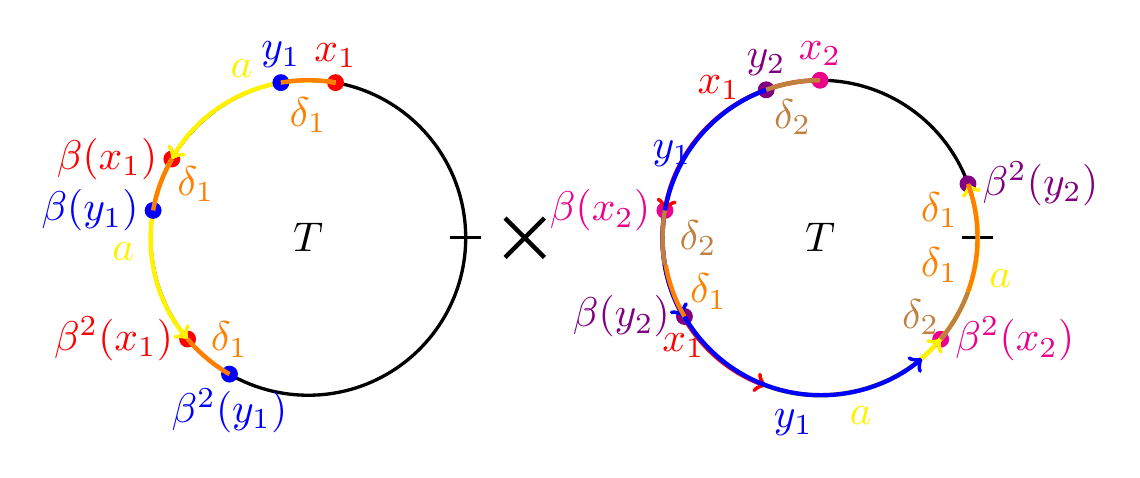
\begin{tikzpicture}
			\draw[very thick] (0, 0) circle (2) node[scale=1.5] {$\mathbb{T}$};
			\draw[very thick] (1.8, 0) -- (2.2, 0);
			
			\onslide<4->\filldraw[color=red] (.347, 1.970) circle (.1) node[anchor=south, scale=1.5] {$x_1$};
			\onslide<5->\filldraw[color=red] (-1.732, 1) circle (.1) node[anchor=east, scale=1.5] {$\beta(x_1)$};
			\onslide<7->\filldraw[color=red] (-1.532, -1.286) circle (.1) node[anchor=east, scale=1.5] {$\beta^2(x_1)$};
			
			\onslide<5-9>\draw[ultra thick, color=yellow, ->] (.347, 1.970) arc (80:150:2) node[above, midway, scale=1.5] {$a$};
			\onslide<7-9>\draw[ultra thick, color=yellow, ->] (-1.732, 1) arc (150:220:2) node[left, midway, scale=1.5] {$a$};
			
			\onslide<9->\filldraw[color=blue] (-.347, 1.970) circle (.1) node[anchor=south, scale=1.5] {$y_1$};
			\onslide<10->\filldraw[color=blue] (-1.970, .347) circle (.1) node[anchor=east, scale=1.5] {$\beta(y_1)$};
			\onslide<14->\filldraw[color=blue] (-1, -1.732) circle (.1) node[anchor=north, scale=1.5] {$\beta^2(y_1)$};
			
			\onslide<9->\draw[ultra thick, color=orange] (.347, 1.970) arc (80:100:2) node[below, midway, scale=1.5] {$\delta_1$};
			\onslide<10->\draw[ultra thick, color=orange] (-1.732, 1) arc(150:170:2) node[right, midway, scale=1.5] {$\delta_1$};
			\onslide<14>\draw[ultra thick, color=orange] (-1.532, -1.286) arc(220:240:2) node[above, scale=1.5] {$\delta_1$};
			
			
			\onslide<1->\draw[ultra thick] (2.5, .25) -- (3, -.25);
			\onslide<1->\draw[ultra thick] (2.5, -.25) -- (3, .25);
			
			
			\onslide<1->\draw[very thick] (6.5, 0) circle (2) node[scale=1.5] {$\mathbb{T}$};
			\onslide<1->\draw[very thick] (8.3, 0) -- (8.7, 0);
			
			\onslide<4->\filldraw[color=magenta] (6.5, 2) circle (.1) node[anchor=south, scale=1.5] {$x_2$};
			\onslide<6->\filldraw[color=magenta] (4.530, .347) circle (.1) node[anchor=east, scale=1.5] {$\beta(x_2)$};
			\onslide<8->\filldraw[color=magenta] (8.032, -1.289) circle (.1) node[anchor=west, scale=1.5] {$\beta^2(x_2)$};
			
			\onslide<6-13>\draw[ultra thick, color=red, ->] (6.5, 2) arc (90:170:2) node[above, midway, scale=1.5] {$x_1$};
			\onslide<8->\draw[ultra thick, color=red, ->] (4.530, .347) arc(170:250:2) node[below, midway, scale=1.5] {$x_1$};
			\onslide<8->\draw[ultra thick, color=yellow, ->] (5.816, -1.879) arc(250:320:2) node[below, midway, scale=1.5] {$a$};
			
			\onslide<9->\filldraw[color=violet] (5.816, 1.879) circle (.1) node[anchor=south, scale=1.5] {$y_2$};
			\onslide<11->\filldraw[color=violet] (4.778, -1) circle (.1) node[anchor=east, scale=1.5] {$\beta(y_2)$};
			\onslide<15->\filldraw[color=violet] (8.379, .684) circle (.1) node[anchor=west, scale=1.5] {$\beta^2(y_2)$};
			
			\onslide<11-12>\draw[ultra thick, color=blue, ->] (5.816, 1.879) arc (110:210:2) node[above, midway, scale=1.5] {$y_1$};
			\onslide<15->\draw[ultra thick, color=blue, ->] (4.778, -1) arc (210:310:2) node[below, midway, scale=1.5] {$y_1$};
			\onslide<15->\draw[ultra thick, color=yellow, ->] (7.786, -1.532) arc(310:380:2) node[right, midway, scale=1.5] {$a$};
			
			\onslide<9->\draw[ultra thick, color=brown] (6.5, 2) arc (90:110:2) node[below, midway, scale=1.5] {$\delta_2$};
			\onslide<12->\draw[ultra thick, color=brown] (4.530, .347) arc (170:190:2) node[right, midway, scale=1.5] {$\delta_2$};
			\onslide<13->\draw[ultra thick, color=orange] (4.778, -1) arc (210:190:2) node[right, midway, scale=1.5] {$\delta_1$};
			\onslide<16->\draw[ultra thick, color=brown] (8.032, -1.289) arc (320:340:2) node[left, midway, scale=1.5] {$\delta_2$};
			\onslide<16->\draw[ultra thick, color=orange] (8.5, 0) arc (360:340:2) node[left, midway, scale=1.5] {$\delta_1$};
			\onslide<17->\draw[ultra thick, color=orange] (8.5, 0) arc(0:20:2) node[left, midway, scale=1.5] {$\delta_1$};
			\onslide<1->
		\end{tikzpicture}
	\end{figure}
\end{frame}

\begin{frame}
	\begin{example}
		The MEF of the skew-ration $(\mathbb{T}^2, \beta)$ is given by the circle rotation $(\mathbb{T}, \alpha)$ with factor map $\pi$ given by $([x_1], [x_2]) \mapsto [x_1]$.\pause
	\end{example}
	We need to prove that
	\begin{align*}
		Q_2(\mathbb{T}^2) = R_\pi = \{(([x_1], [x_2]), ([y_1], [y_2])) \in \mathbb{T}^2 \times \mathbb{T}^2;\ [x_1] = [y_1]\}.
	\end{align*}\pause

	We already know that $(\mathbb{T}, \alpha)$ is equicontinuous, which implies $Q_2(\mathbb{T}^2) \subseteq R_\pi$.
\end{frame}

\begin{frame}
	For the other direction we prove that $(([z], [x]), ([z], [y])) \in R_\pi$ is regional proximal.
	\medskip
	
	\onslide<3->{Fix $\varepsilon > 0$. W.l.o.g. $0 \leq x \leq y < 1$.} \onslide<4->{Choose some $0 < b < \frac{\varepsilon}{2}$ and $n \in \mathbb{N}$ such that
	\begin{align*}
		\textcolor<10>{blue}{0 < (y-x) - nb} < \frac{\varepsilon}{2}.
	\end{align*}}
	\onslide<5->{Then $([z+b], [x])$ and $([z], [y])$ are in the $\varepsilon$ balls around $([z], [x])$ and $([z], [y])$ and}
	\begin{align*}
		\onslide<6->{&d_{\mathbb{T}^2}(\beta^n([z+b], [x]), \beta^n([z], [y]))}\\
		\onslide<8->{= &d_{\mathbb{T}^2}((\textcolor<9>{blue}{[z+b+na]}, \textcolor<10>{blue}{[x + n(z+b) + \frac{n(n+1)}{n}a]}), (\textcolor<9>{blue}{[z+na]}, \textcolor<10>{blue}{[y + nz + \frac{n(n+1)}{2}a]}))}\\
		\onslide<9->{\leq &\textcolor<9>{blue}{b} + \textcolor<10>{blue}{x - y - nb}} \onslide<11->{< \frac{\varepsilon}{2} + \frac{\varepsilon}{2}} \onslide<12->{= \varepsilon}
	\end{align*}
	\begin{overlayarea}{\textwidth}{2cm}
	\begin{minipage}{\textwidth}
		\only<2-6>{
		\begin{definition}[Regional Proximal]
			Two points $x,y \in X$ are called \emph{regionally proximal}
			if for each $\varepsilon > 0$ there exist $x' \in B_\varepsilon(x), y' \in B_\varepsilon(y)$ and $t \in T$ such that $d(tx', ty') < \varepsilon$.
		\end{definition}}
		\only<7->{
		\begin{remark}
			Note that for $([z], [x]) \in \mathbb{T}^2$ and $n \in \mathbb{N}$ we have
			\begin{align*}
				\beta^n([z], [x]) = ([z+na], [x + nz + \frac{n(n-1)}{2}a]).
			\end{align*}
		\end{remark}}
	\end{minipage}
	\end{overlayarea}
\end{frame}